\chapter{किसी स्तनधारी का कार्यात्मक संगठन}\label{ch:b1:mammal-organization}

विच्छेदन-पटल पर किसी खरगोश को खोलिए और पहला प्रभाव व्यवस्था का पड़ता है।
एक पेशीय चादर, \omterm{def:b1:mammal-organization:bodyplan}{मध्यपट}, धड़ को दो भागों में बाँटती है: एक वक्ष, जिसमें
हृदय और दो फेफड़े हैं, और एक उदर, जिसमें बाक़ी सब --- मुट्ठी भर का यकृत,
एक आमाशय, चार मीटर आँत जो आमाशय जितने बड़े अंधनाल पर जाकर समाप्त होती है,
और पिछली भित्ति से सटे दो गुर्दे। हर \omterm{def:b1:mammal-organization:organ}{अंग} की एक जगह है, एक रक्त-आपूर्ति है
और एक काम; इनमें से कोई अकेले काम नहीं करता। यह अध्याय बताता है कि
स्तनधारी एक कार्यरत समग्र के रूप में कैसे बना है: उसकी \omterm{def:b1:mammal-organization:bodyplan}{शरीर-योजना}, वे
तंत्र जिनमें उसके \omterm{def:b1:mammal-organization:organ}{अंग} समूहबद्ध हैं, वे द्रव-कक्ष जिनमें उसकी कोशिकाएँ
रहती हैं, वे \omterm{prop:b1:organism-environment:surfaces}{विनिमय सतहें} जिनसे वह बाहर से मिलता है, और वह ऊष्मीय संतुलन
जो उसे जनवरी के मैदान में \qty{39}{\celsius} पर बनाए रखता है।

\section{किसी स्तनधारी की शरीर-योजना}

\begin{definition}[शरीर-योजना]\label{def:b1:mammal-organization:bodyplan}
किसी जंतु की \emph{शरीर-योजना}\index{शरीर-योजना} उसके अक्षों, गुहाओं और
\omterm{def:b1:mammal-organization:organ}{अंगों} की वह सजावट है जो उसके समूह के सभी सदस्यों में साझा होती है।
स्तनधारी की शरीर-योजना किसी कशेरुकी की है: द्विपार्श्व सममिति, जिसमें एक
शिरोभाग मस्तिष्क और मुख्य ज्ञानेंद्रियाँ धारण करता है
(\emph{शीर्षीभवन}\index{शीर्षीभवन}), कशेरुकों का एक पृष्ठीय अक्ष जो
मेरुरज्जु को घेरता है, चार उपांग, और एक अधर देहगुहा ---
\emph{देहगुहा}\index{देहगुहा} --- जिसमें अंतरंग \omterm{def:b1:mammal-organization:organ}{अंग} रहते हैं। जो विशेष
रूप से स्तनधारी का है वह यह: देहगुहा पेशीय \emph{मध्यपट}\index{मध्यपट}
से एक वक्षीय गुहा (हृदय, फेफड़े) और एक उदरीय गुहा (पाचन \omterm{def:b1:mammal-organization:organ}{अंग}, गुर्दे,
जनद) में बँटी होती है; शरीर बालों से ढका होता है; शावक दूध पर पलते हैं;
और ताप नियंत्रित होता है।
\end{definition}

\begin{omfigure}
\begin{tikzpicture}
  \node[anchor=south west, inner sep=0] (img) at (0,0)
    {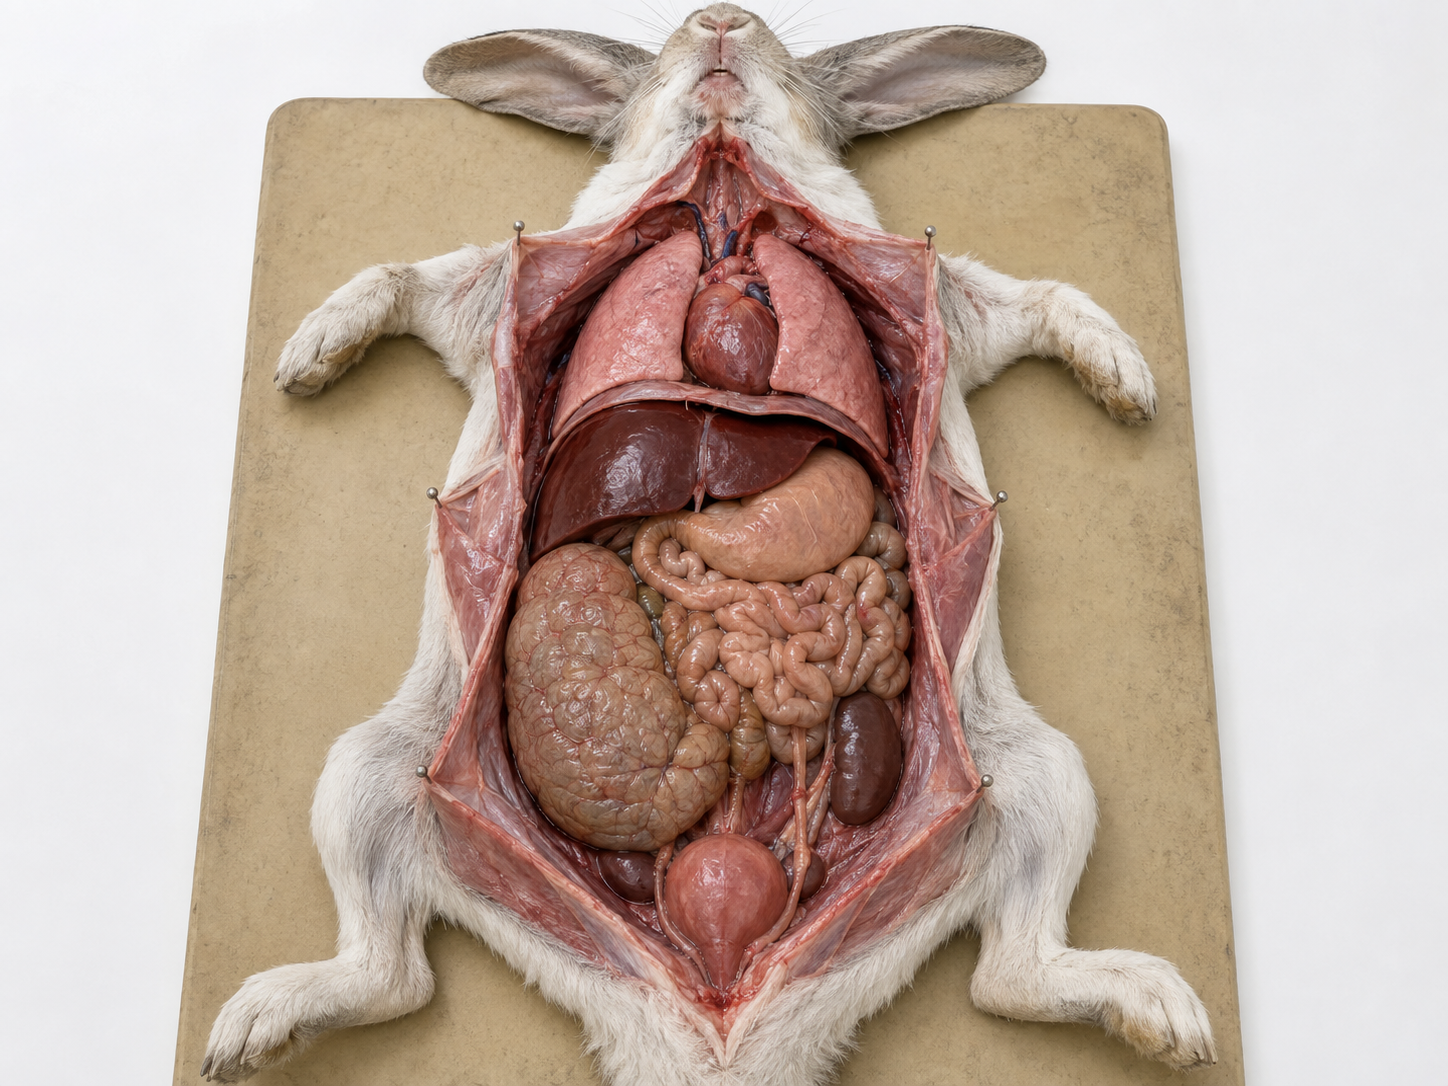
\includegraphics[width=0.6\linewidth]{images/book3/ai/fig-rabbit-dissection.png}};
  \begin{scope}[x={(img.south east)}, y={(img.north west)},
      every node/.style={font=\small}]
    \draw[omDef, thick] (0.44,0.72) -- (-0.02,0.90) node[left] {फेफड़े};
    \draw[omDef, thick] (0.50,0.68) -- (1.02,0.88) node[right] {हृदय};
    \draw[omDef, thick] (0.53,0.61) -- (1.02,0.70) node[right] {मध्यपट};
    \draw[omDef, thick] (0.44,0.55) -- (-0.02,0.62) node[left] {यकृत};
    \draw[omDef, thick] (0.56,0.52) -- (1.02,0.54) node[right] {आमाशय};
    \draw[omDef, thick] (0.52,0.42) -- (1.02,0.40) node[right] {छोटी आँत};
    \draw[omDef, thick] (0.42,0.36) -- (-0.02,0.36) node[left] {अंधनाल};
    \draw[omDef, thick] (0.60,0.30) -- (1.02,0.24) node[right] {गुर्दा};
    \draw[omDef, thick] (0.51,0.17) -- (-0.02,0.10) node[left] {मूत्राशय};
  \end{scope}
\end{tikzpicture}

{\small अधर की ओर से खोला गया एक खरगोश। \omterm{def:b1:mammal-organization:bodyplan}{मध्यपट} वक्षीय गुहा (फेफड़े,
हृदय) को उदरीय गुहा (यकृत, आमाशय, आँत, अंधनाल, गुर्दे, मूत्राशय) से
अलग करती है। हर \omterm{def:b1:mammal-organization:organ}{अंग} एक नियत जगह पर है, एक झिल्ली में लिपटा है और अपनी
ही वाहिकाओं से पोषित है।}
\end{omfigure}

\begin{definition}[अंग, अंग तंत्र]\label{def:b1:mammal-organization:organ}
\emph{अंग}\index{अंग} कई ऊतकों (\cref{ch:b1:body-plans-tissues}) से बनी
वह संरचना है जो किसी निश्चित कार्य के लिए सजी हो: हृदय पंप करता है,
फेफड़ा गैसों का विनिमय करता है, गुर्दा छानता है। \emph{अंग
तंत्र}\index{अंग तंत्र} एक व्यापक कार्य में सहयोग करते अंगों का समुच्चय
है: पाचन तंत्र मुँह से गुदा तक चलता है और उससे यकृत तथा अग्न्याशय जुड़े
हैं; परिसंचरण तंत्र हृदय और वाहिकाएँ हैं; उत्सर्जन तंत्र गुर्दे और मूत्र
मार्ग।
\end{definition}

\section{अंग तंत्र और वे कार्य जो वे साधते हैं}

\begin{proposition}[कार्यों के तीन समूह]\label{prop:b1:mammal-organization:functions}
किसी स्तनधारी के \omterm{def:b1:mammal-organization:organ}{अंग तंत्र} कार्यों के तीन समूह साधते हैं:
\begin{itemize}
  \item \emph{पोषण}\index{पोषण कार्य}: पदार्थ और ऊर्जा भीतर लेना और
        बाँटना तथा अपशिष्ट निकालना --- पाचन, श्वसन, परिसंचरण और
        उत्सर्जन तंत्र;
  \item \emph{संबंध}\index{संबंध कार्य}: पर्यावरण को भाँपना और उस पर
        क्रिया करना --- ज्ञानेंद्रियाँ, तंत्रिका तंत्र, अंतःस्रावी
        ग्रंथियाँ, कंकाल और पेशियाँ;
  \item \emph{जनन}\index{जनन कार्य}: संतति पैदा करना --- जनद, जनन मार्ग
        और, स्तनधारियों में, स्तन ग्रंथियाँ।
\end{itemize}
कोई तंत्र अकेले काम नहीं करता: हर \omterm{def:b1:mammal-organization:organ}{अंग} आपूर्ति के लिए रक्त पर, समन्वय के
लिए तंत्रिका तथा अंतःस्रावी तंत्रों पर, और रक्षा के लिए कंकाल तथा त्वचा
पर निर्भर है।
\end{proposition}

\begin{omfigure}
\begin{tikzpicture}[font=\footnotesize, >=Stealth, line cap=round,
  sys/.style={draw, thick, rounded corners=3pt, minimum height=7mm, minimum width=24mm, align=center, fill=white},
  lab/.style={font=\scriptsize, above},
  grp/.style={font=\small\bfseries, anchor=west}]
  \node[grp, omProp] at (0,4.6) {पोषण};
  \node[sys, fill=omProp!12] (dig) at (1.3,3.8) {पाचन};
  \node[sys, fill=omProp!12] (res) at (1.3,2.9) {श्वसन};
  \node[sys, fill=omProp!12] (exc) at (1.3,2.0) {उत्सर्जन};
  \node[grp, omExo] at (0,1.1) {जनन};
  \node[sys, fill=omExo!12] (gen) at (1.3,0.3) {जनन मार्ग};
  \node[sys, fill=omThm!12, minimum height=30mm] (cir) at (5.9,2.6) {परिसंचरण\\ (रक्त, लसीका)};
  \node[grp, omDef] at (8.6,4.6) {संबंध};
  \node[sys, fill=omDef!12, minimum width=30mm] (ner) at (10.3,3.8) {तंत्रिका, इंद्रियाँ};
  \node[sys, fill=omDef!12, minimum width=30mm] (end) at (10.3,2.9) {अंतःस्रावी};
  \node[sys, fill=omDef!12, minimum width=30mm] (mus) at (10.3,2.0) {कंकाल, पेशियाँ};
  \node[sys, fill=omDef!12, minimum width=30mm] (ski) at (10.3,1.1) {त्वचा};
  \draw[<->, thick] (dig.east) -- (cir.west |- dig.east) node[lab, midway] {पोषक तत्व};
  \draw[<->, thick] (res.east) -- (cir.west |- res.east) node[lab, midway] {$\mathrm{O_2}$, $\mathrm{CO_2}$};
  \draw[<->, thick] (exc.east) -- (cir.west |- exc.east) node[lab, midway] {अपशिष्ट};
  \draw[<->, thick] (gen.east) -- ++(1.6,0) |- (cir.south west);
  \draw[<->, thick] (cir.east |- ner.west) -- (ner.west);
  \draw[<->, thick] (cir.east |- end.west) -- (end.west) node[lab, midway] {हॉर्मोन};
  \draw[<->, thick] (cir.east |- mus.west) -- (mus.west);
  \draw[<->, thick] (cir.south east) -| ++(0.5,0) |- (ski.west);
\end{tikzpicture}

{\small किसी स्तनधारी के \omterm{def:b1:mammal-organization:organ}{अंग तंत्र}, कार्य के अनुसार समूहबद्ध। परिसंचरण
ही धुरी है: हर तंत्र रक्त से विनिमय करता है, और जो एक तंत्र भीतर लेता है
उसे रक्त हर दूसरे तंत्र तक पहुँचा देता है।}
\end{omfigure}

\begin{example}[घास का एक कौर]\label{ex:b1:mammal-organization:mouthful}
खरगोश की घास कृंतकों से कटती है और चर्वणकों से पिसती है (कंकाल और
पेशियाँ), चखी और सूँघी जाती है (इंद्रियाँ), निगली जाती है और आमाशय तथा
छोटी आँत में पचती है; उसकी शर्कराएँ और ऐमीनो अम्ल आँत की भित्ति पार कर
रक्त में जाते हैं और यकृत तक पहुँचते हैं, जो उन्हें हॉर्मोनी नियंत्रण
में संचित करता है या छोड़ता है (अंतःस्रावी); उसका सेलुलोस अंधनाल में
जीवाणुओं से किण्वित होता है; शर्कराएँ जलाने की ऑक्सीजन फेफड़ों से आती है,
कार्बन डाइऑक्साइड उसी रास्ते जाती है, ऐमीनो अम्लों से बना यूरिया गुर्दों
से जाता है, और पूरी प्रक्रिया की ऊष्मा त्वचा से। एक कौर के लिए सात
तंत्र।
\end{example}

\section{शरीर के कक्ष}

\begin{definition}[द्रव-कक्ष]\label{def:b1:mammal-organization:compartments}
जल किसी स्तनधारी के द्रव्यमान का लगभग \qty{60}{\%} है। उसका दो-तिहाई
\emph{अंतःकोशिकीय द्रव}\index{अंतःकोशिकीय द्रव} है, कोशिकाओं के भीतर;
एक-तिहाई \emph{बाह्यकोशिकीय द्रव}\index{बाह्यकोशिकीय द्रव} है, यानी
\cref{ch:b1:organism-environment} का \omterm{def:b1:organism-environment:milieu}{आंतरिक पर्यावरण}, जो स्वयं
कोशिकाओं को नहलाते \emph{अंतराली द्रव}\index{अंतराली द्रव} (उसका
तीन-चौथाई) और वाहिकाओं के भीतर के \emph{रक्त
प्लाज़्मा}\index{प्लाज़्मा} (एक-चौथाई) में बँटा है। \emph{लसीका}\index{लसीका}
वह अंतराली द्रव है जिसे लसीका वाहिकाएँ इकट्ठा करके रक्त में लौटाती हैं।
दोनों बाह्यकोशिकीय द्रवों का संघटन लगभग एक ही है --- प्लाज़्मा अपने
प्रोटीनों से भिन्न है, जो केशिका भित्ति पार नहीं करते --- और दोनों
अंतःकोशिकीय द्रव से तीखे रूप से भिन्न हैं।
\end{definition}

\begin{omfigure}
\begin{tikzpicture}[font=\small, line cap=round]
  \draw[thick, fill=gray!8, rounded corners=6pt] (0,0) rectangle (11.6,4.6);
  \node[anchor=north west, font=\small\bfseries] at (0.15,4.55) {शरीर का कुल जल: \qty{42}{L} (\qty{70}{kg} का \qty{60}{\%})};
  \draw[thick, fill=omDef!14, rounded corners=5pt] (0.3,0.3) rectangle (6.4,3.8);
  \node[anchor=north west, align=left] at (0.4,3.7) {\textbf{अंतःकोशिकीय द्रव}: \qty{28}{L}\\ उच्च $\mathrm{K^+}$ (\qty{140}{mmol/L}),\\ फ़ॉस्फ़ेट, प्रोटीन;\\ निम्न $\mathrm{Na^+}$ (\qty{10}{mmol/L})};
  \draw[thick, fill=omProp!14, rounded corners=5pt] (6.7,0.3) rectangle (11.3,3.8);
  \node[anchor=north west, align=left] at (6.8,3.7) {\textbf{बाह्यकोशिकीय द्रव}: \qty{14}{L}\\ उच्च $\mathrm{Na^+}$ (\qty{140}{mmol/L}),\\ $\mathrm{Cl^-}$, $\mathrm{HCO_3^-}$};
  \draw[thick, fill=omProp!30, rounded corners=4pt] (6.9,0.45) rectangle (9.2,1.55);
  \node[align=center, font=\footnotesize] at (8.05,1.0) {अंतराली\\ \qty{11}{L}};
  \draw[thick, fill=omThm!30, rounded corners=4pt] (9.4,0.45) rectangle (11.1,1.55);
  \node[align=center, font=\footnotesize] at (10.25,1.0) {प्लाज़्मा\\ \qty{3}{L}};
\end{tikzpicture}

{\small \qty{70}{kg} के मनुष्य के द्रव-कक्ष। जल का दो-तिहाई कोशिकाओं के
भीतर है; बाह्यकोशिकीय तिहाई, जो \omterm{def:b1:mammal-organization:compartments}{अंतराली द्रव} और प्लाज़्मा में बँटा है,
\omterm{def:b1:organism-environment:milieu}{आंतरिक पर्यावरण} है। बाहर सोडियम का बोलबाला है और भीतर पोटैशियम का --- यह
अंतर बनाए रखने में हर कोशिका ऊर्जा ख़र्च करती है
(\cref{ch:b1:membranes-transport})।}
\end{omfigure}

\begin{method}[तनूकरण से किसी कक्ष का मापन]\label{met:b1:mammal-organization:dilution}
\begin{enumerate}
  \item ऐसा सूचक चुनिए जो उसी कक्ष में फैले और कहीं नहीं: प्लाज़्मा के
        लिए प्लाज़्मा प्रोटीनों से बँधा कोई रंजक (इवांस नीला);
        \omterm{def:b1:mammal-organization:compartments}{बाह्यकोशिकीय द्रव} के लिए इनुलिन, यानी वह शर्करा जो वाहिकाओं से
        बाहर तो जाती है पर कोशिकाओं में नहीं घुसती; और शरीर के कुल जल के
        लिए भारी जल।
  \item ज्ञात मात्रा $m$ भीतर डालिए और मिश्रण होने की प्रतीक्षा कीजिए
        (प्लाज़्मा के लिए मिनट, कुल जल के लिए घंटे)।
  \item प्लाज़्मा के किसी नमूने में सांद्रता $c$ मापिए, और प्रतीक्षा के
        दौरान हुई किसी भी हानि (मूत्र, उपापचय) के लिए संशोधन कीजिए।
  \item आयतन $V = m/c$ है। अंतःकोशिकीय आयतन कुल जल में से बाह्यकोशिकीय
        घटाने पर मिलता है; अंतराली आयतन बाह्यकोशिकीय में से प्लाज़्मा
        घटाने पर। रक्त का आयतन प्लाज़्मा के आयतन को रक्त के प्लाज़्मा
        भिन्न ($1 - $ रक्तकणिका-मात्रा) से भाग देने पर मिलता है।
\end{enumerate}
\end{method}

\begin{example}[एक प्लाज़्मा आयतन]\label{ex:b1:mammal-organization:evansblue}
\qty{70}{kg} के किसी पुरुष में डाला गया \qty{50}{mg} इवांस नीला दस मिनट
बाद \qty{16.7}{mg/L} की प्लाज़्मा सांद्रता देता है:
$V = 50/16.7 = \qty{3.0}{L}$ प्लाज़्मा। \qty{45}{\%} की
रक्तकणिका-मात्रा के साथ रक्त का आयतन $3.0/0.55 = \qty{5.5}{L}$ है ---
यानी शरीर के द्रव्यमान का \qty{8}{\%}, और यह अनुपात चूहे से व्हेल तक
टिकता है।
\end{example}

\section{विनिमय सतहें और परिसंचरण}

\begin{proposition}[हर विनिमय सतह रक्त से युग्मित है]\label{prop:b1:mammal-organization:surfaces}
कोई स्तनधारी बाहर से चार सतहों से विनिमय करता है, जिनमें से हर एक शरीर
के भीतर मुड़ी है और हर एक सघन केशिका-जाल से पोषित: पोषक तत्वों और जल के
लिए आँत की श्लेष्मा (मनुष्य में \qty{30}{m^2}), ऑक्सीजन और कार्बन
डाइऑक्साइड के लिए फेफड़ों की कूपिका-सतह (\qty{100}{m^2}), अपशिष्टों और
\omterm{def:b1:organism-environment:milieu}{आंतरिक पर्यावरण} के नियमन के लिए गुर्दों की छानने वाली सतह (दस लाख
कोशिकागुच्छ, जो दिन में \qty{180}{L} प्लाज़्मा छानते हैं), और ऊष्मा तथा
थोड़े जल के लिए त्वचा (\qty{2}{m^2})। परिसंचरण इन्हें जोड़ता है: एक सतह
से चला रक्त एक मिनट के भीतर अगली सतह पर पहुँच जाता है, ताकि जो आँत से
भीतर आता है वह फेफड़े की ऑक्सीजन से ऑक्सीकृत हो और उसका अपशिष्ट गुर्दे
से बाहर जाए।
\end{proposition}

\begin{omfigure}
\begin{tikzpicture}[font=\small, >=Stealth, line cap=round,
  org/.style={draw, thick, rounded corners=4pt, minimum height=8mm, minimum width=22mm, align=center, fill=white}]
  \node[org, fill=omDef!12] (lung) at (0,3.2) {फेफड़े\\ \qty{100}{m^2}};
  \node[org, fill=omThm!15, minimum width=26mm, minimum height=12mm] (heart) at (0,0) {हृदय\\ दायाँ $\mid$ बायाँ};
  \node[org, fill=omProp!12] (gut) at (5.2,1.6) {आँत\\ \qty{30}{m^2}};
  \node[org, fill=omProp!12] (liver) at (5.2,0.0) {यकृत};
  \node[org, fill=omProp!12] (kid) at (5.2,-1.6) {गुर्दे\\ \qty{180}{L/d}};
  \node[org, fill=omExo!12] (mus) at (5.2,3.2) {पेशियाँ, त्वचा,\\ मस्तिष्क, अन्य};
  % pulmonary loop
  \draw[->, very thick, omDef] (heart.north west) ++(-0.2,0) |- (lung.west) node[pos=0.25, left, font=\footnotesize, align=right] {फुफ्फुस\\ परिपथ};
  \draw[->, very thick, omThm] (lung.east) -| ($(heart.north east)+(0.2,0)$);
  % systemic loop: left heart -> organs (parallel) -> right heart
  \draw[very thick, omThm] (heart.east) -- ++(1.2,0) coordinate (a);
  \draw[->, very thick, omThm] (a) |- (mus.west);
  \draw[->, very thick, omThm] (a) |- (gut.west);
  \draw[->, very thick, omThm] (a) |- (kid.west);
  \draw[->, very thick, omThm] (a) -- (liver.west);
  \draw[->, very thick, omDef] (gut.south) -- (liver.north) node[midway, right, font=\footnotesize] {निवाहिका शिरा};
  \coordinate (b) at (8.0,0.8);
  \draw[very thick, omDef] (mus.east) -| (b);
  \draw[very thick, omDef] (liver.east) -| (b);
  \draw[very thick, omDef] (kid.east) -| (b);
  \draw[->, very thick, omDef] (b) |- ++(0,-3.2) -| (heart.south) node[pos=0.25, below, font=\footnotesize] {दैहिक परिपथ: शिराएँ};
\end{tikzpicture}

{\small किसी स्तनधारी का दोहरा परिसंचरण। दायाँ हृदय ऑक्सीजन-दरिद्र रक्त
(नीला) फेफड़ों से भेजता है; बायाँ हृदय ऑक्सीजनित रक्त (लाल) \omterm{def:b1:mammal-organization:organ}{अंगों} से
भेजता है, जो समांतर में सजे हैं, ताकि हर \omterm{def:b1:mammal-organization:organ}{अंग} को ताज़ा धमनी-रक्त मिले।
आँत से आया रक्त हृदय लौटने से पहले यकृत से होकर जाता है।}
\end{omfigure}

\begin{omfigure}
\begin{tikzpicture}
\begin{axis}[
  xbar, bar width=8pt,
  width=0.82\linewidth, height=6.2cm,
  axis x line=bottom, axis y line=left,
  xmin=0, xmax=1.8, xlabel={विश्राम में रक्त-प्रवाह (\unit{L/min})},
  xlabel style={font=\small, at={(axis description cs:0.5,-0.13)}, anchor=north},
  symbolic y coords={heart muscle, skin, brain, skeletal muscle, kidneys, liver and gut},
  yticklabels={हृदय पेशी, त्वचा, मस्तिष्क, कंकाल पेशी, गुर्दे, यकृत और आँत},
  ytick=data, tick label style={font=\small},
  enlarge y limits=0.12, xtick={0,0.5,1.0,1.5},
  nodes near coords, nodes near coords style={font=\scriptsize, anchor=west},
]
\addplot[fill=omThm!45, draw=omThm] coordinates
  {(0.25,heart muscle) (0.4,skin) (0.75,brain) (1.0,skeletal muscle) (1.1,kidneys) (1.35,liver and gut)};
\end{axis}
\end{tikzpicture}

{\small विश्राम में \qty{5}{L/min} के मानव हृदय-निर्गम का \omterm{def:b1:mammal-organization:organ}{अंगों} में
बँटवारा। गुर्दे, जो शरीर के द्रव्यमान का \qty{0.5}{\%} हैं, रक्त का
पाँचवाँ भाग लेते हैं --- यह पूरे प्लाज़्मा को दिन में साठ बार छानने की
क़ीमत है। व्यायाम के दौरान पेशियों का हिस्सा दस गुना बढ़ जाता है और आँत
का घट जाता है।}
\end{omfigure}

\begin{example}[परिसंचरण-काल]\label{ex:b1:mammal-organization:circtime}
\qty{5.5}{L} रक्त और \qty{5}{L/min} के हृदय-निर्गम के साथ रक्त की एक
बूँद विश्राम में दोहरा परिपथ लगभग एक मिनट में पूरा करती है, और कड़े
व्यायाम में उसका एक-चौथाई समय लेती है, जब निर्गम \qty{20}{L/min} तक
पहुँच जाता है। हृदय-निर्गम $M^{3/4}$ की तरह बदलता है
(\cref{thm:b1:organism-environment:kleiber}): \qty{2}{kg} के खरगोश का
निर्गम \qty{160}{mL} रक्त के लिए लगभग \qty{0.35}{L/min} है --- यानी दो
के गुणक के भीतर वही परिसंचरण-काल, और वह भी प्रति मिनट \qty{200}{} धड़कन
की हृदय-दर पर।
\end{example}

\section{अंतस्तापिता और ऊष्मीय संतुलन}

\begin{proposition}[ऊष्मा-बजट]\label{prop:b1:mammal-organization:heatbudget}
\index{ऊष्मा-बजट}
स्थिर ताप पर कोई स्तनधारी इसे संतुष्ट करता है
\[
M - W = R + C + K + E ,
\]
जिसमें $M$ उपापचयी ऊष्मा-उत्पादन है, $W$ बाहर पर किया गया यांत्रिक कार्य,
और दायाँ पक्ष विकिरण $R$, हवा में संवहन $C$, ज़मीन में चालन $K$ और वाष्पन
$E$ (फेफड़ों से, तथा पसीने या हाँफने से) द्वारा होने वाली हानियाँ। पहली
तीन हानियाँ $T_b - T_a$ के समानुपाती हैं और उन्हें रोमों की कुचालकता तथा
त्वचा में रक्त-प्रवाह चलाते हैं; वाष्पन ही एकमात्र मार्ग है जो हवा के
शरीर से गरम होने पर भी काम करता है। जब समीकरण संतुष्ट नहीं होता, तब शरीर
का ताप उस दर से खिसकता है जो असंतुलन और शरीर की ऊष्माधारिता (लगभग
\qty{3.5}{kJ.kg^{-1}.K^{-1}}) से तय होती है।
\end{proposition}
\begin{proof}
शरीर के लिए ऊर्जा-संरक्षण, उस अवधि में जिसमें उसका ताप नहीं बदलता:
मुक्त हुई रासायनिक ऊर्जा ($M$) या तो कार्य के रूप में जाती है या चार
भौतिक मार्गों से ऊष्मा के रूप में। $R$, $C$, $K$ का ताप-अंतर के साथ
समानुपाती होना न्यूटन का शीतलन नियम है
(\cref{ch:b1:organism-environment}); और $E$ का उस अंतर से स्वतंत्र होना
इससे निकलता है कि वाष्पन को आर्द्रता की प्रवणता चलाती है, ताप की प्रवणता
नहीं।
\end{proof}

\begin{omfigure}
\begin{tikzpicture}[font=\small, >=Stealth, line cap=round]
  \draw[very thick, fill=omThm!8, rounded corners=16pt] (0,0) rectangle (5.0,3.0);
  \node[align=center] at (2.5,1.5) {देह-अंतर्भाग \qty{39}{\celsius}\\ ऊष्मा-उत्पादन $M$\\ (आधारी, कँपकँपी, क्रिया)};
  \draw[->, very thick, omThm] (5.0,2.5) -- (6.6,2.5) node[right, align=left] {$R$: दीवारों और आकाश की ओर विकिरण};
  \draw[->, very thick, omThm] (5.0,1.8) -- (6.6,1.8) node[right, align=left] {$C$: हवा में संवहन};
  \draw[->, very thick, omThm] (5.0,1.1) -- (6.6,1.1) node[right, align=left] {$K$: ज़मीन में चालन};
  \draw[->, very thick, omDef] (5.0,0.4) -- (6.6,0.4) node[right, align=left] {$E$: वाष्पन (साँस, पसीना)};
  \draw[->, very thick, omExo] (-1.6,1.5) -- (0,1.5) node[pos=0, left, align=right] {भोजन की ऊर्जा\\ (और संचित वसा)};
  \draw[->, very thick, gray] (2.5,0) -- (2.5,-0.9) node[below, align=center] {$W$: बाहर पर कार्य};
  \node[font=\footnotesize, align=center, anchor=south] at (2.5,3.1) {रोम और त्वचा का रक्त-प्रवाह $R$, $C$, $K$ तय करते हैं;\\ ये $\propto (T_b - T_a)$ हैं};
\end{tikzpicture}

{\small किसी \omterm{prop:b1:organism-environment:thermo}{अंतस्तापी} का \omterm{prop:b1:mammal-organization:heatbudget}{ऊष्मा-बजट}। उत्पादन को चारों हानियों तथा बाहरी
कार्य के योग के बराबर होना चाहिए; जंतु संतुलन बनाए रखने के लिए उत्पादन
(कँपकँपी, क्रिया), कुचालकता (रोम, मुद्रा, त्वचा का रक्त-प्रवाह) और
वाष्पन को समायोजित करता है।}
\end{omfigure}

\begin{proposition}[तापनियमन के साधन]\label{prop:b1:mammal-organization:thermoreg}
ठंड के विरुद्ध स्तनधारी हानि घटाता है --- रोम खड़े करके, त्वचा तथा
सिरों की वाहिकाएँ सिकोड़कर, सिकुड़कर, झुंड में सटकर --- और उत्पादन
बढ़ाता है: कँपकँपी (पेशियों का लयबद्ध संकुचन) और, छोटे तथा नवजात
स्तनधारियों में, \emph{भूरे वसा ऊतक}\index{भूरा वसा ऊतक} में
\emph{अकंपन ऊष्माजनन}\index{अकंपन ऊष्माजनन}, जिसकी सूत्रकणिकाएँ वसा की
ऊर्जा सीधे ऊष्मा के रूप में छोड़ती हैं। गरमी के विरुद्ध वह त्वचा की
वाहिकाएँ फैलाता है (खरगोश के कान उसकी एक-तिहाई ऊष्मा बहा सकते हैं), और
पसीने (घोड़ा, मनुष्य) या हाँफने (कुत्ता, खरगोश) से जल का वाष्पन करता है।
यह सब हाइपोथैलेमस से संचालित होता है, जो \omterm{def:b1:organism-environment:homeostasis}{नियत बिंदु} रखता है और रक्त तथा
त्वचा का ताप पढ़ता है।
\end{proposition}
\begin{proof}[साक्ष्य]
किसी कुत्ते के हाइपोथैलेमस को रोपे गए प्रोब से गरम करने पर वह ठंडे कमरे
में भी हाँफता है और अपनी त्वचा की वाहिकाएँ फैलाता है; प्रोब को ठंडा करने
पर वह गरम कमरे में भी काँपता है। \qty{5}{\celsius} पर रखे किसी मूषक की
ऑक्सीजन-खपत एक घंटे के भीतर तिगुनी हो जाती है, जिसमें आधी वृद्धि कँपकँपी
से आती है (पेशी की विद्युत क्रिया के रूप में अभिलिखित) और आधी भूरी वसा
से, जिसका ताप तापयुग्म से मापने पर आसपास के ऊतकों से अधिक निकलता है।
\qty{30}{\celsius} पर किसी खरगोश के अवरक्त चित्र उसके कानों को लगभग
शरीर के ताप पर दिखाते हैं, और \qty{5}{\celsius} पर लगभग हवा के ताप पर।
\end{proof}

\begin{example}[खरगोश के कान]\label{ex:b1:mammal-organization:ears}
लगभग \qty{50}{cm^2} के दो कान, पतले, लगभग नंगे और ख़ूब रक्त-पूरित:
\qty{20}{\celsius} की हवा में \qty{30}{\celsius} पर उनकी वाहिकाएँ खुली
हों और नंगी त्वचा का गुणांक \qty{10}{W.m^{-2}.K^{-1}} हो, तो वे
$10\times 0.01\times 10 =
\qty{1}{W}$ खोते हैं, जो विश्राम कर रहे खरगोश के उत्पादन का छठा भाग है। \qty{5}{\celsius} पर वाहिकाएँ बंद हो जाती हैं,
कान ठंडे होकर लगभग हवा के ताप पर आ जाते हैं, और उनसे होने वाली हानि
\qty{0.2}{W} से नीचे गिर जाती है।
\end{example}

\begin{remark}[समन्वय]\label{rem:b1:mammal-organization:coordination}
ऊपर का हर समायोजन --- किसी वाहिका का सँकरा होना, किसी पेशी का काँपना,
किसी ग्रंथि का स्रावित करना --- कोई तंत्रिका या हॉर्मोन ले जाता हुआ आदेश
है। तंत्रिका तंत्र नियत तारों के सहारे मिलीसेकंडों में काम करता है;
अंतःस्रावी तंत्र रक्त के माध्यम से मिनटों से घंटों में काम करता है और उस
हर कोशिका तक पहुँचता है जो सही ग्राही धारण करती है। उनकी क्रियाविधियाँ
वर्ष 2 के खंड का विषय हैं; यह वर्ष उन्हें दिया हुआ मानकर चलता है और यह
पढ़ता है कि वे किसका समन्वय करती हैं।
\end{remark}

\section{अभ्यास}

\begin{exercise}[$\star$]\label{exo:b1:mammal-organization:1}
स्तनधारी की \omterm{def:b1:mammal-organization:bodyplan}{शरीर-योजना} के वे लक्षण गिनाइए जो सभी कशेरुकियों में साझा
हैं, और वे जो केवल स्तनधारियों के अपने हैं।
\end{exercise}

\begin{exercise}[$\star$]\label{exo:b1:mammal-organization:2}
हर \omterm{def:b1:mammal-organization:organ}{अंग तंत्र} को कार्यों के तीन समूहों में से किसी एक में रखिए, और हर
तंत्र का एक \omterm{def:b1:mammal-organization:organ}{अंग} बताइए।
\end{exercise}

\begin{exercise}[$\star$]\label{exo:b1:mammal-organization:3}
\qty{60}{kg} की कोई स्त्री: उसके शरीर का कुल जल, उसके अंतःकोशिकीय और
बाह्यकोशिकीय आयतन, उसका अंतराली आयतन और उसका प्लाज़्मा आयतन आँकिए।
\end{exercise}

\begin{exercise}[$\star$]\label{exo:b1:mammal-organization:4}
रक्त-प्रवाह वाले आलेख से बताइए कि हृदय-निर्गम का कितना भिन्न गुर्दों को
जाता है, और रक्त का पूरा आयतन (\qty{5.5}{L}) दिन में कितनी बार उनसे
होकर पंप होता है।
\end{exercise}

\begin{exercise}[$\star\star$]\label{exo:b1:mammal-organization:5}
\qty{70}{kg} के किसी पुरुष में \qty{2.0}{g} इनुलिन डाला जाता है; मिश्रण
हो जाने के बाद, और \qty{0.3}{g} मूत्र में चले जाने के बाद, प्लाज़्मा
सांद्रता \qty{0.12}{g/L} है। बाह्यकोशिकीय आयतन निकालिए, और कुल जल
\qty{42}{L} लेकर अंतःकोशिकीय आयतन भी।
\end{exercise}

\begin{exercise}[$\star\star$]\label{exo:b1:mammal-organization:6}
समझाइए कि प्लाज़्मा और \omterm{def:b1:mammal-organization:compartments}{अंतराली द्रव} का आयनिक संघटन एक ही क्यों है पर
प्रोटीन की मात्रा में वे भिन्न क्यों हैं, और यदि प्लाज़्मा प्रोटीन खो
जाएँ तो अंतराली आयतन का क्या होगा।
\end{exercise}

\begin{exercise}[$\star\star$]\label{exo:b1:mammal-organization:7}
दैहिक परिपथ के \omterm{def:b1:mammal-organization:organ}{अंग} शृंखला में क्यों नहीं, समांतर में क्यों रखे गए हैं?
मस्तिष्क को पेशियों के नीचे-प्रवाह में रखने का क्या परिणाम होता?
\end{exercise}

\begin{exercise}[$\star\star$]\label{exo:b1:mammal-organization:8}
\qty{20}{\celsius} की हवा में विश्राम कर रहा कोई मनुष्य
($M = \qty{80}{W}$, $W = 0$) फेफड़ों और त्वचा से वाष्पन द्वारा
\qty{20}{W} खोता है। यदि विकिरण, संवहन और चालन मिलकर
$hS(T_b - T_a)$ हों, जिसमें $S = \qty{1.8}{m^2}$ और $T_b$ (त्वचा) $=
\qty{33}{\celsius}$, तो $h$ निकालिए। हवा के \qty{33}{\celsius} पर पहुँच
जाने पर त्वचा के ताप का क्या होता है?
\end{exercise}

\begin{exercise}[$\star\star$]\label{exo:b1:mammal-organization:9}
व्यायाम कर रहा कोई मनुष्य \qty{800}{W} बनाता है और \qty{200}{W} बाहरी
कार्य करता है। अवाष्पनी हानियाँ \qty{150}{W} हैं। ताप स्थिर रखने के लिए
प्रति घंटे कितना जल वाष्पित होना चाहिए (गुप्त ऊष्मा
\qty{2.4}{kJ/g})? यदि पसीना रुक जाए तो ताप कितनी तेज़ी से बढ़ेगा
(\qty{70}{kg}, \qty{3.5}{kJ.kg^{-1}.K^{-1}})?
\end{exercise}

\begin{exercise}[$\star\star\star$]\label{exo:b1:mammal-organization:10}
नवजात स्तनधारी और छोटी जातियाँ कँपकँपी के बजाय भूरी वसा पर निर्भर रहती
हैं। सतह-आयतन अनुपात और हर क्रियाविधि की प्रकृति की सहायता से दो कारण
सुझाइए।
\end{exercise}

\begin{exercise}[$\star\star\star$]\label{exo:b1:mammal-organization:11}
किसी कुत्ते के हाइपोथैलेमस को प्रोब से गरम किया जाता है जबकि कुत्ता ठंडे
कमरे में बैठा है। उसकी अनुक्रियाओं की, और एक घंटे बाद उसके अंतर्भाग के
ताप की भविष्यवाणी कीजिए। फिर उस कुत्ते की अनुक्रियाओं की भविष्यवाणी
कीजिए जिसका हाइपोथैलेमस नष्ट है और जिसे बारी-बारी से ठंडे और गरम कमरे
में रखा जाता है।
\end{exercise}

\begin{exercise}[$\star\star\star$]\label{exo:b1:mammal-organization:12}
``\omterm{def:b1:organism-environment:milieu}{आंतरिक पर्यावरण} स्तनधारी का निजी समुद्र है।'' इस बिंब पर एक अनुच्छेद
में चर्चा कीजिए: \omterm{def:b1:mammal-organization:compartments}{बाह्यकोशिकीय द्रव} क्या है, उसे अचर कौन रखता है, और कौन
से \omterm{def:b1:mammal-organization:organ}{अंग तंत्र} उसके तट हैं।
\end{exercise}

\section{समस्या: खरगोश का एक दिन}

\begin{problem}[{सप्ताहांत समस्या --- जनवरी में दो किलोग्राम के एक
खरगोश के चौबीस घंटे: उसकी ऊर्जा, उसका जल, उसका रक्त और उसकी ऊष्मा, और
अंत में उसका दैनिक ऊर्जा-व्यय तथा जल-आवर्तन}]
\label{pb:b1:mammal-organization:1}
किसी जंगली खरगोश का द्रव्यमान \qty{2.0}{kg} है और शरीर का ताप
\qty{39}{\celsius}। उसकी \omterm{def:b1:organism-environment:allometry}{आधारी उपापचय दर} क्लाइबर के नियम का पालन करती
है, $B = \qty{3.4}{W}\,(M/\qty{1}{kg})^{3/4}$। उसका दिन: \qty{12}{h}
अपने बिल में विश्राम, अपने \omterm{prop:b1:organism-environment:thermo}{तापउदासीन क्षेत्र} के भीतर; \qty{6}{h} चराई,
अपनी आधारी दर के तीन गुने पर; और \qty{6}{h} बाहर \qty{5}{\celsius} पर
विश्राम, जहाँ उसे अपनी आधारी दर का दुगुना बनाना पड़ता है। वह हरी घास
खाता है जिसमें \qty{25}{\%} शुष्क पदार्थ है; शुष्क पदार्थ में
\qty{18}{kJ/g} है, जिसका वह \qty{65}{\%} पचाता है।

\medskip
\noindent\textbf{भाग I --- ऊर्जा।}
\begin{enumerate}
  \item खरगोश की \omterm{def:b1:organism-environment:allometry}{आधारी उपापचय दर} वाट में निकालिए।
  \item तीनों अवधियों में से हर एक में ख़र्च हुई ऊर्जा किलोजूल में
        निकालिए।
  \item दैनिक ऊर्जा-व्यय निकालिए और उसे \qty{24}{h} की आधारी दर के
        गुणज के रूप में लिखिए।
  \item एक ग्राम हरी घास की पाच्य ऊर्जा निकालिए।
  \item प्रतिदिन खाई गई हरी घास का द्रव्यमान निकालिए, और उसमें निहित
        शुष्क पदार्थ का द्रव्यमान भी।
  \item हरे भोजन के ग्रहण को शरीर-द्रव्यमान के भिन्न के रूप में लिखिए।
  \item खपी हुई ऑक्सीजन के प्रति लीटर \qty{20}{kJ} लेकर दैनिक
        ऑक्सीजन-खपत और उसकी माध्य दर मिलीलीटर प्रति मिनट में निकालिए।
  \item $0.9$ के श्वसन गुणांक (प्रति लीटर $\mathrm{O_2}$ पर लीटर
        $\mathrm{CO_2}$) के साथ दैनिक कार्बन डाइऑक्साइड निर्गम लीटर
        में और ग्राम में निकालिए (\qty{22.4}{L/mol},
        \qty{44}{g/mol})।
\end{enumerate}

\medskip
\noindent\textbf{भाग II --- जल।}
पचे हुए शुष्क पदार्थ का ऑक्सीकरण प्रति ग्राम \qty{0.6}{g} उपापचयी जल
देता है। बिना पचा शुष्क पदार्थ मल के साथ जाता है, जो \qty{40}{\%} जल
होता है। मूत्र प्रतिदिन \qty{130}{mL} है। खरगोश दिन में \qty{860}{L}
हवा साँस लेता है; वह \qty{10}{\celsius} की हवा भीतर लेता है जिसमें
\qty{5}{g/m^3} जलवाष्प है, और \qty{37}{\celsius} पर संतृप्त हवा बाहर
छोड़ता है, \qty{44}{g/m^3}। त्वचा से वाष्पन दिन में \qty{20}{g} है।
\begin{enumerate}[resume]
  \item घास के साथ भीतर आया जल निकालिए।
  \item बनी हुई उपापचयी जल की मात्रा निकालिए।
  \item मल का द्रव्यमान और उसके साथ जाने वाला जल निकालिए।
  \item साँस में खोया जल निकालिए।
  \item जल का बहीखाता बनाइए: कुल आगम, कुल निर्गम, और उनका अंतर।
  \item क्या खरगोश को पानी पीना पड़ेगा? उस अंतर का क्या होता है?
  \item अगस्त में घास \qty{50}{\%} शुष्क पदार्थ होती है। उसी
        ऊर्जा-ग्रहण के लिए भोजन का जल फिर से निकालिए, और निष्कर्ष
        दीजिए।
\end{enumerate}

\medskip
\noindent\textbf{भाग III --- रक्त और कक्ष।}
\begin{enumerate}[resume]
  \item अध्याय के भिन्नों की सहायता से खरगोश के शरीर का कुल जल,
        बाह्यकोशिकीय आयतन और प्लाज़्मा आयतन निकालिए।
  \item \qty{1.5}{mg} इवांस नीला डाला जाता है; मिश्रण के बाद प्लाज़्मा
        सांद्रता \qty{15}{mg/L} है। प्लाज़्मा आयतन निकालिए और आकलन से
        तुलना कीजिए।
  \item \qty{40}{\%} की रक्तकणिका-मात्रा के साथ रक्त का आयतन निकालिए।
  \item हृदय-निर्गम \qty{70}{kg} पर \qty{5}{L/min} के मानव मान से
        $M^{3/4}$ की तरह बदलता है। खरगोश का हृदय-निर्गम निकालिए और वह
        समय भी जो रक्त की एक बूँद को परिपथ पूरा करने में लगता है।
  \item प्रति मिनट \qty{200}{} धड़कन की हृदय-दर के साथ आघात-आयतन
        निकालिए।
\end{enumerate}

\medskip
\noindent\textbf{भाग IV --- ऊष्मा।}
खरगोश की सतह $S = \qty{0.1}{m^2}\,(M/\qty{1}{kg})^{2/3}$ है; उसके रोम
$h = \qty{2.5}{W.m^{-2}.K^{-1}}$ देते हैं; और हर कान लगभग नंगी त्वचा का
\qty{50}{cm^2} है जिसके लिए $h = \qty{10}{W.m^{-2}.K^{-1}}$ है।
\begin{enumerate}[resume]
  \item खरगोश की सतह निकालिए।
  \item \qty{5}{\celsius} पर रोमों से खोई ऊष्मा निकालिए और बाहर की
        अवधि के लिए मानी गई उत्पादन-दर से उसकी तुलना कीजिए।
  \item दोनों कानों से होने वाली हानि निकालिए, पहले जब उनकी वाहिकाएँ
        खुली हों (त्वचा \qty{39}{\celsius} पर) और फिर जब बंद हों (त्वचा
        \qty{8}{\celsius} पर)। जनवरी में खरगोश क्या करता है?
  \item अगस्त में, \qty{30}{\celsius} पर, रोमों से और खुले कानों से
        होने वाली हानि निकालिए, और उनके योग की तुलना आधारी उत्पादन से
        कीजिए। खरगोश \qty{39}{\celsius} पर कैसे बना रहता है?
  \item परिणाम बताइए: खरगोश का दैनिक ऊर्जा-व्यय मेगाजूल में और उसकी
        आधारी दर के गुणज के रूप में, तथा उसका दैनिक जल-आवर्तन ग्राम में
        और अपने द्रव्यमान के भिन्न के रूप में।
\end{enumerate}
\end{problem}
